
\subsection{Definición y Descripción de un Robot}


La realidad es que, lo que hoy día consideramos , no se asemeja a lo que en sus inicios se llamaba robot. Pero sí que existen características generales que nos permiten llamar de la misma forma a los robot que se empezaban a desarrollar desde la antigua Grecia, y que naturalmente eran muy rudimentarios, y a los robot que conocemos hoy día y que ayudan notablemente a facilitar la vida diaria de las personas.\\

Si nos limitamos a definiciones como pueden ser de la R.A.E. se dice que un robot es \textit{"Máquina o ingenio electrónico programable, capaz de manipular objetos y realizar operaciones antes reservadas solo a las personas."} Además, un robot también debe de contar con las siguientes características:

\begin{itemize}
\item \textbf{Multifuncionalidad:} Capaz de llevar a cabo varias tareas.
\item \textbf{Programable:} Capaz de modificar su funcionalidad sin un excesivo costo.
\item \textbf{Alto Grado de Autonomía:} Capaz de ejecutar su tarea sin la intervención de un humano.
\end{itemize}

Pero nada más leer esta definición nos damos cuenta que no es válida para los robots que se describirán a continuación ya que alrededor del año 400 a.C. no se podía hablar de máquinas programables y mucho menos electrónicas. La realidad es que el concepto de robots tal y como se conoce hoy en día, no se desarrolló hasta 1948 de la mano de George Devol. Más adelante se explicará con mayor profundidad la importancia de este en la historia de la robótica.\\

A modo de curiosidad, la palabra \textit{robot} tiene su origen en la obra teatral \textit{Robots Universales Rossum} dirigida por un dramaturgo checo que se estrenó en 1920. Es por tanto, que no fue hasta 1920 cuando comenzó a llamarse \textit{robot} a todo lo que vamos a describir en próximos apartados.

\subsection{Orígenes de la Robótica (Griegos)}

Los primeros autómatas se desarrollaron en el Antiguo Egipcio. Como es natural estos no tienen nada que ver con lo que hoy se conoce como autómata, pero tenía bastante mérito para la época a la que pertenecen. Eso sí, se consideraban como tales ya que eran capaces de realizar determinadas tareas de forma autónoma. A continuación se van a mencionar los robots más relevantes de la época:\\

 \textbf{Arquitas de Tarento} en el año 400 a.C. diseñó \textit{"la paloma"}[\ref{paloma}], ave mecánica que funcionaba con vapor. El mecanismo era muy rudimentario, debido a la época, y funcionaba de la siguiente manera; Se trataba de un objeto de madera con forma de paloma que se situaba colgada de una cuerda del techo. Esta contenía un pequeño depósito de agua, que se llevaba a ebullición mediante una llama situada en la parte inferior del depósito, y el vapor que se originaba se filtraba por unos pequeños orificios que le permitían al "\textit{robot}" simular el vuelo de la paloma.\\
 
\begin{figure}[H]
\begin{center}
  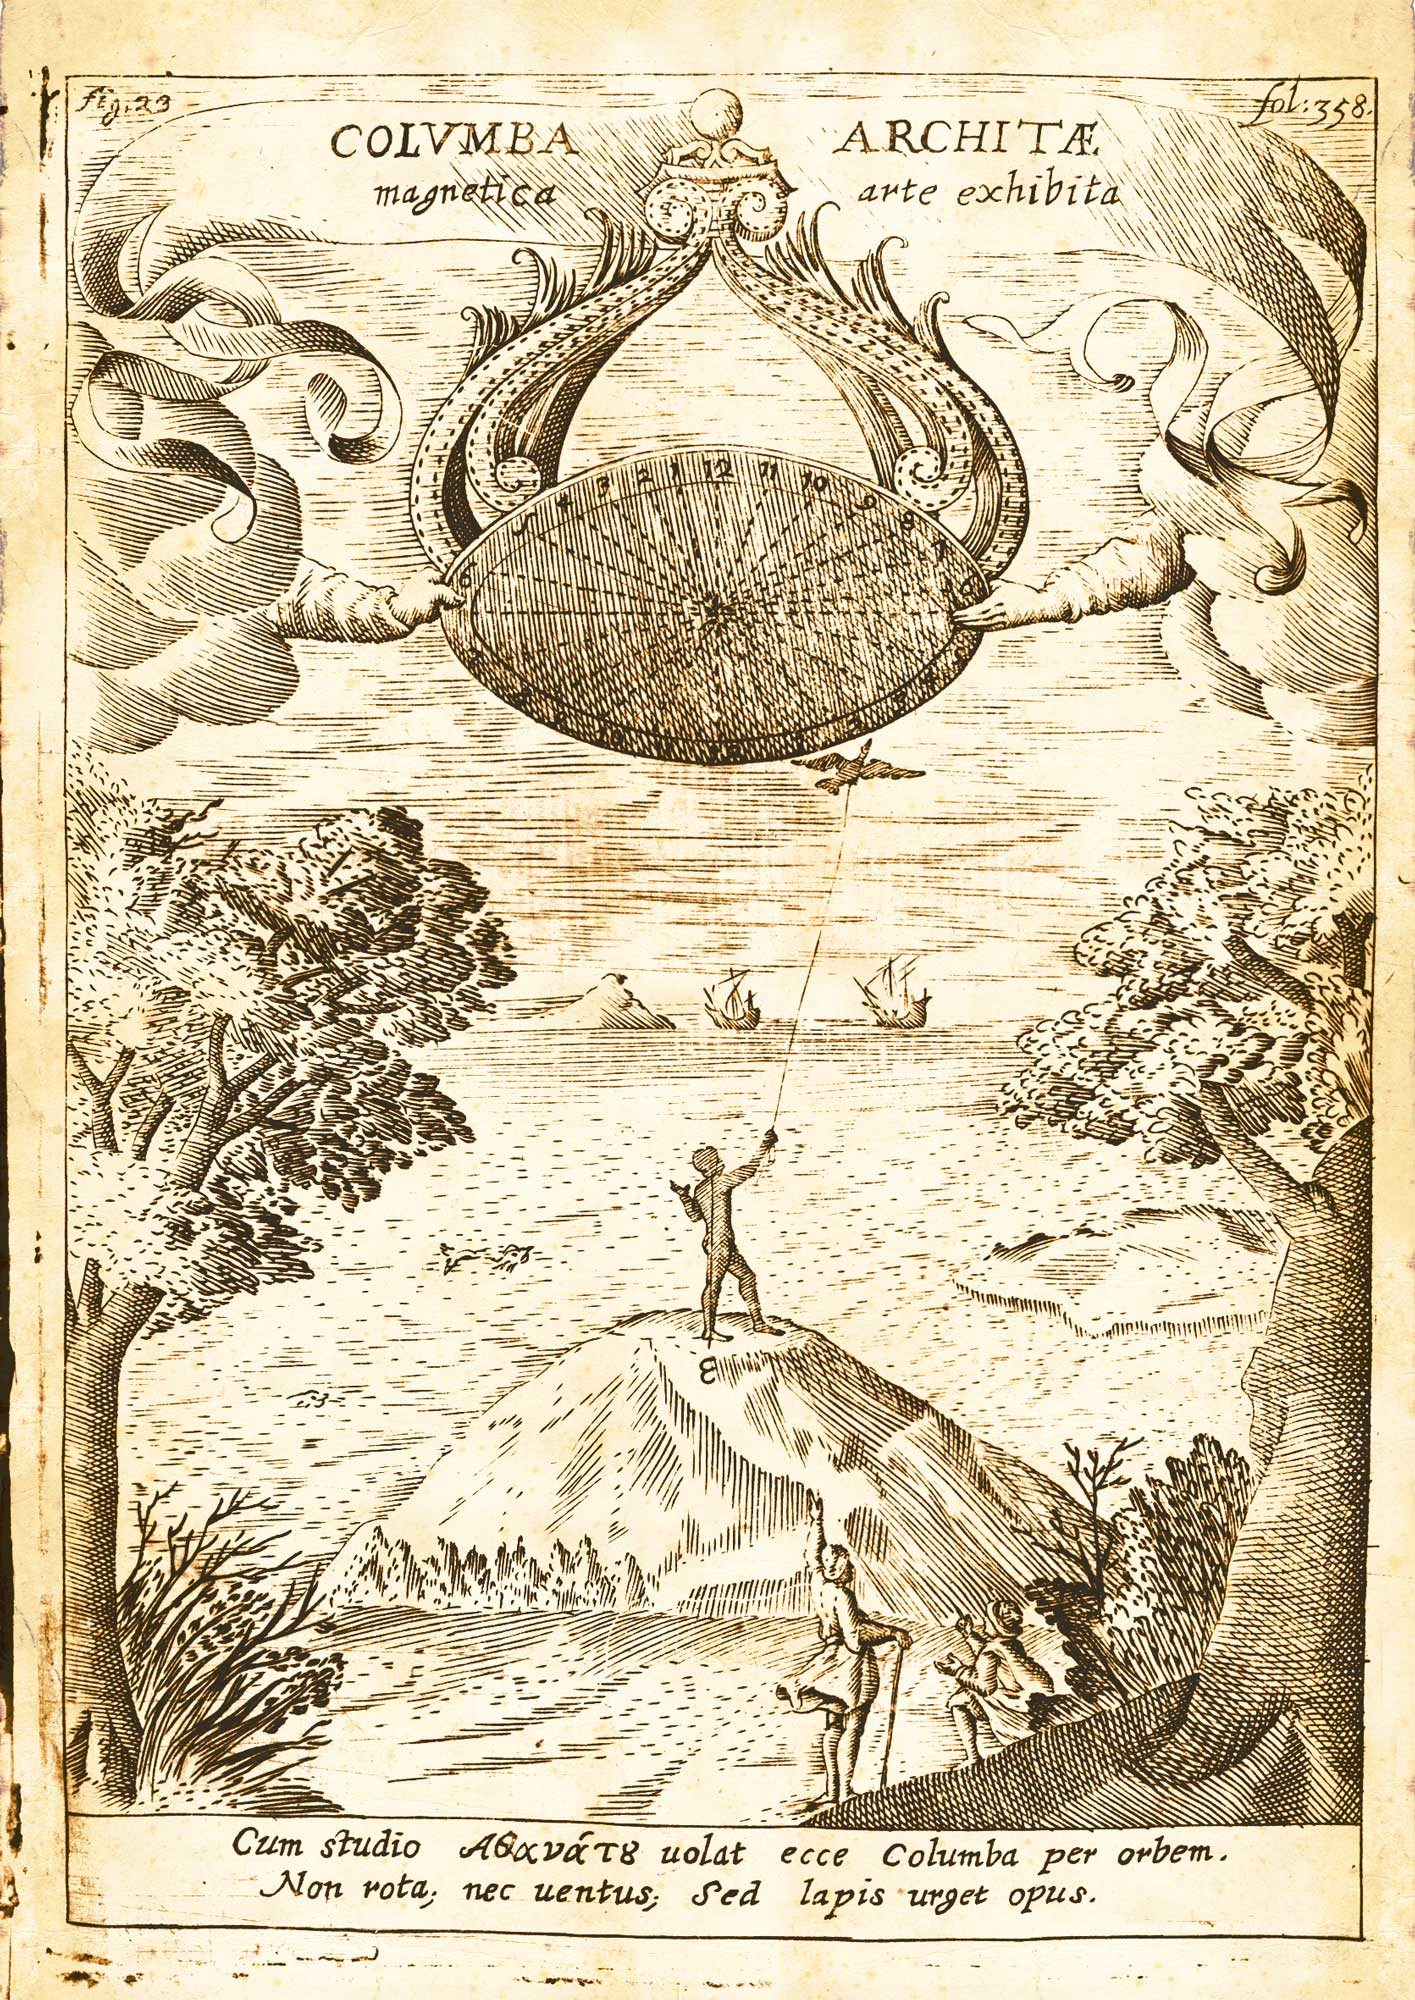
\includegraphics[width=0.5\textwidth]{./EtapaPrimeriza/imagenes/paloma.jpg}
  \caption{Paloma de Arquitas de Tarento (\href{https://www.nationalgeographic.com.es/historia/grandes-reportajes/inventos-griegos_9395/3}{NationalGeographic})}
  \label{paloma}
\end{center}
\end{figure}


\textbf{Apolonio de Pérgamo}, entre 262-190 a.C. , diseñó unos autómatas musicales que funcionaban impulsados por la fuerza del agua.\\


\textbf{Ctesibio de Alejandría}, en el año 300 a.C., también inventó autómatas musicales pero en este caso funcionaban por la propulsión de aire a través de diversos tubos. Pero su contribución más relevante fue el desarrollo del \textit{reloj de agua o clepsidra}, este fue el más preciso de los relojes creados hasta la aparición del reloj de péndulo. Tenía la capacidad de medir el tiempo en función de lo que tarda en caer el agua de un recipiente a otro. Hasta ese momento, el tiempo se medía el tiempo a través de la observación del movimiento del sol, lo que no permitía medir el tiempo en cualquier momento del día. A continuación se muestra una imagen de dicho reloj:\\

	
\begin{figure}[H]
\begin{center}
  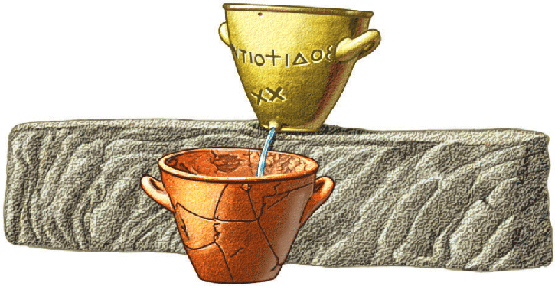
\includegraphics[width=0.5\textwidth]{./EtapaPrimeriza/imagenes/reloj.png}
  \caption{Reloj de Agua de Ctesibio de Alejandría (\href{http://quhist.com/origen-a-lo-largo-historia-termino-clepsidra/}{QuHist})}
  \label{reloj}
\end{center}
\end{figure}



\textbf{Filón de Bizancio} inventa en el año 200 a. C., hizo numerosas contribuciones a la ciencia que se describirán a continuación. Uno de los inventos más revolucionarios fue el molino de agua que se utilizaba tanto para moler grano como para diversos trabajos agrícolas. Además, ideó la bomba de agua que permitía transportar el agua desde un nacimiento hasta una zona geográficamente más alta mediante la fuerza de la propia agua. Relacionado también con el agua, ideó un lavabo en el que, como se puede ver en la siguiente imagen, contenía en su parte superior un recipiente lleno de agua. Esta agua caía sobre un cucharón situado bajo el mismo y cuando se llenaba se inclinaba y el agua caía sobre el grifo y pudiendo obtenerla de forma dosificada. Al mismo tiempo que el agua caía por el grifo, también se dejaba caer una pequeña piedra pómez para limpiarte.\\


\begin{figure}[H]
\begin{center}
  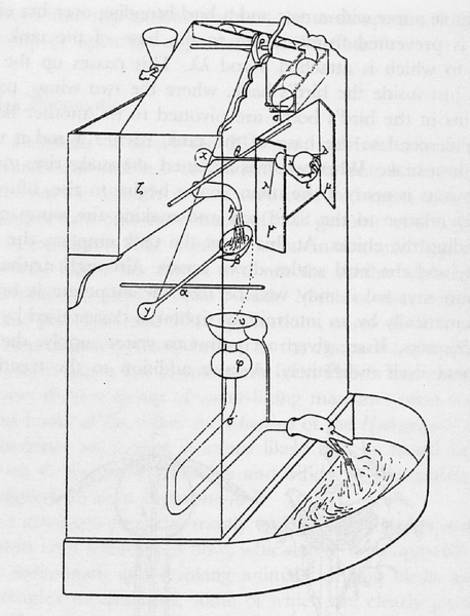
\includegraphics[width=0.3\textwidth]{./EtapaPrimeriza/imagenes/lavabo.jpg}
  \caption{Lavabo de Filón de Bizancio (\href{http://historiautomatas.blogspot.com/2010/06/grecia-ii-filon-de-bizancio.html} {HistoriaAutómatas})}
  \label{lavabo}
\end{center}
\end{figure}

Pero estas no fueron las únicas contribuciones de Filón de Bizancio. Tenía cierto interés por el tema armamentístico y es por ello que diseñó las primeras flechas, una ballesta que está compuesta por dos cadenas unidas con una polea tal que se lanzaban flechas mientras le quedaran en la recámara. Y por último, y uno de sus inventos más curiosos fue lo que se llamó una \textit{camarera automática}. Esto era una estatua que tenía colocada en una de sus manos una jarra y cuando se le colocaba en la otra mano un vaso, esta cedía por el peso y el tubo que conectaba la jarra con el depósito del vino se accionaba para llenar el vaso. 



\textbf{Herón de Alejandría} destaca por las numerosas contribuciones que hizo a la ciencia en la antigüedad. Es por ello que se va a hacer desarrollar sus contribuciones más relevantes y algunas de ellas han facilitado avances industriales a lo largo de la historia.

En sus contribuciones a lo que podría ser la robótica de la época se destaca su trabajo conocido como \textit{Mecánica}, en el que se plasman los primeros datos descriptivos acerca de la construcción de un autómata. Está compuesto por tres libros en los que se trata de las proporciones de las figuras en el primero de ellos, en el segundo de los sistemas mecánicos simples que son descritos en el siguiente apartado y finalmente en su último libro hablaba sobre las aplicaciones de la mecánica.

Cuando hablamos de inventos concretos se destaca que creó la primera máquina de vapor de la historia a la que llamaron \textit{eolípila}. Esta estaba compuesta por una caldera de agua hirviendo y sobre esta se situaba una esfera hueca llena de agua conectadas ambas cosas por dos tubos como se ve en la siguiente imagen [\ref{mv}]. Cuando el agua hervía se conseguía que la esfera girase a gran velocidad. En la época se dice que solo servía como un divertimento para los niños pero la realidad es que en el futuro serviría como inspiración a las máquinas de vapor utilizadas en las industrias.

\begin{figure}[H]
\begin{center}
  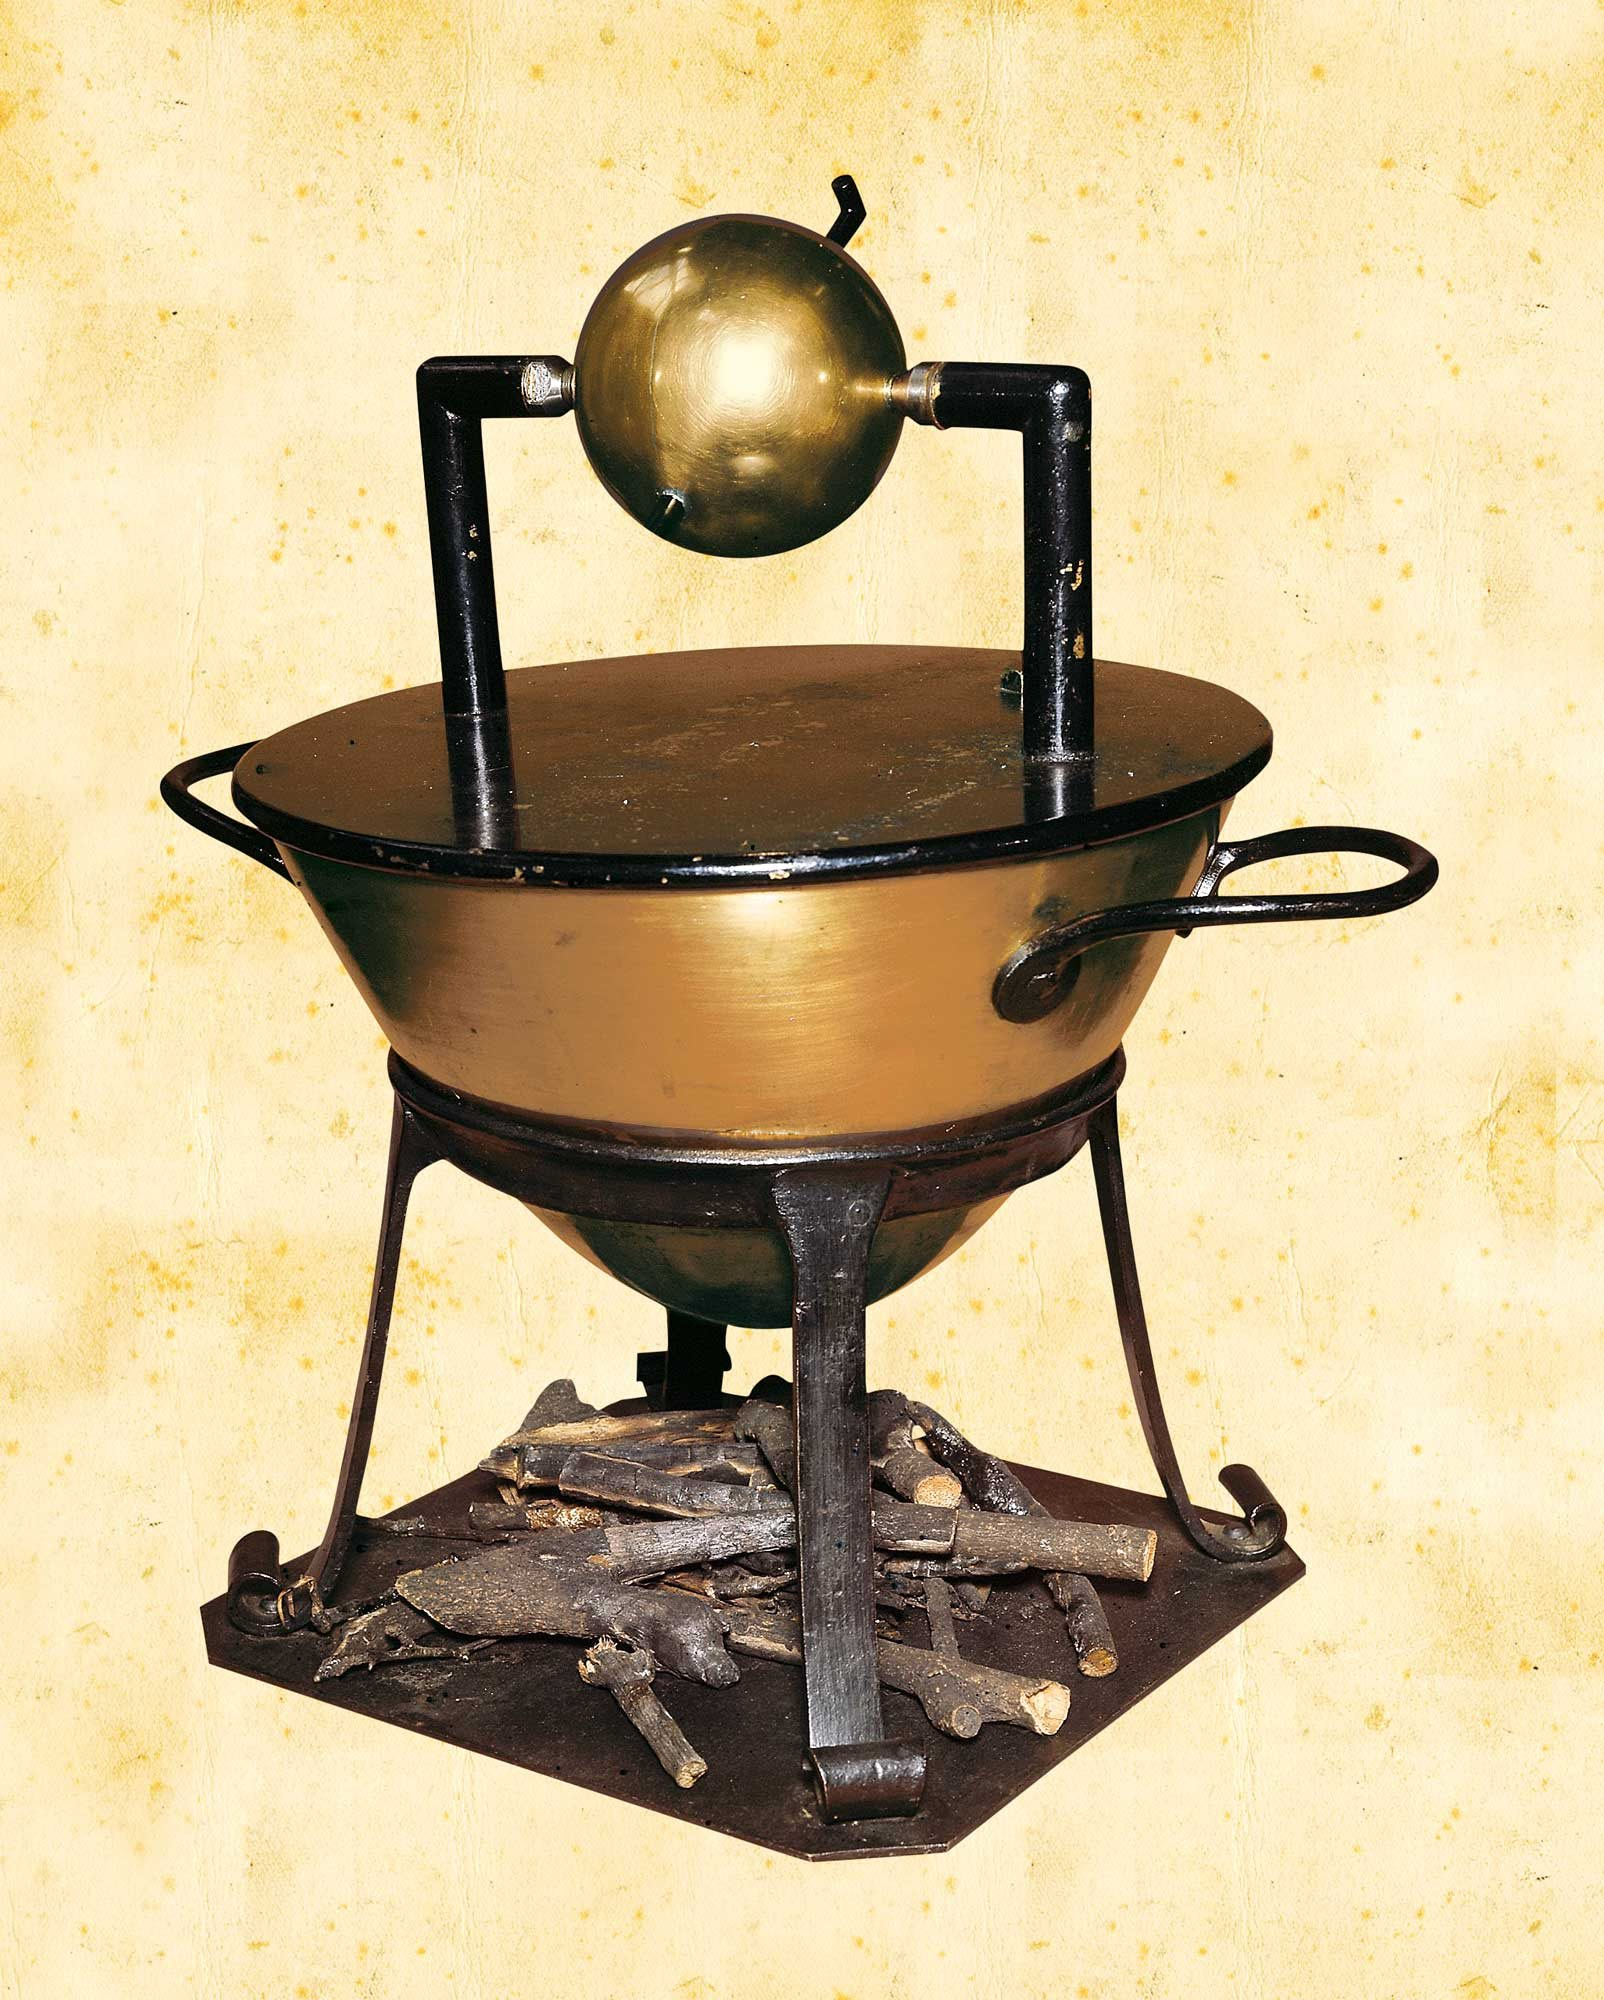
\includegraphics[width=0.3\textwidth]{./EtapaPrimeriza/imagenes/mv.jpg}
  \caption{Eolípila de Herón (\href{https://www.nationalgeographic.com.es/historia/grandes-reportajes/inventos-griegos\_9395}{NationalGeographic})}
  \label{mv}
\end{center}
\end{figure}

Además diseñó lo que fueron los primeros autómatas y las primeras puertas automáticas. Con la energía que proporcionaba la \textit{eolípila} y con sistemas mecánicos simples como cuerdas, poleas, cadenas y demás era capaz de poner en movimiento autómatas y puertas automáticas. La realidad es que no existe constancia de que lo llevara acabo pero la idea si que la tuvo y dejó constancia de ello en sus libros.\\


En el 770 d. C., \textbf{Yang Wu-Lien } diseñó un prototipo con forma de mono que alargaba la mano para que le dieran limosna. Cuando la mano alcanzaba un cierto peso, este guardaba el dinero en una bolsa.\\



En el 890, \textbf{Han Chih Ho} creó un gato de madera que se encargaba de cazar ratas y ratones que hubiese a su alrededor.\\

El príncipe hindú \textbf{Bhoja}, en el año 1050, escribió \textit{Samarangana-Sutradhara} donde se describe cómo es el proceso de construcción de máquinas que eran capaces de actuar autónomamente y que se las llamaba \textit{yantras}.\\


Pero la realidad es que, en la antigüedad, las máquinas más perfectas que se consiguieron fueron los relojes ya que se acercaban al concepto de automatismo y por consiguiente al de robótica. Algunos de ellos cuentan con figuras humanas que sus movimientos van en función del transcurso de las horas. Ejemplos de ello son los relojes de la catedral de Múnich y el reloj de Ánker que se puede visitar en la ciudad de Viena, Austria.

Más concretamente, en España se conserva un reloj construido en el siglo XVI, llamado Papamoscas,  y que está compuesto por un hombre que se mueve con los cambios horarios. Hoy en día sigue funcionado y se puede visitar en la catedral de Burgos.


Aunque se ha de señalar que el robot más antiguo, que estuvo en funcionamiento entre 1352 y 1789, y que se conserva en la actualidad es el Gallo de Estrasburgo. Este formaba era parte del reloj de la catedral de Estrasburgo y hacía mover sus alas y su pico al dar las horas.

\begin{figure}[H]
\begin{center}
  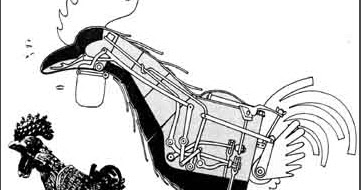
\includegraphics[width=0.3\textwidth]{./EtapaPrimeriza/imagenes/gallo.jpg}
  \caption{Gallo de Estrasburgo  (\href{http://lasmilrespuestas.blogspot.com/2012/06/como-funcionaban-los-automatas.html} {Autómatas})}
  \label{gallo}
\end{center}
\end{figure}


Finalmente, para terminar con los orígenes de la robótica no podemos dejar de nombrar "\textit{el hombre de hierro}" de Alberto Magno del siglo XIII. Este era un autómata con forma de humano construido con hierro, cristal y cuero y que era capaz caminar, abrir puertas, entretener invitados y hasta incluso hacer tareas del hogar. Este es considerado como el inicio de lo que hoy en día es la inteligencia artificial.


\subsection{Sistemas Mecánicos Simples}

Cuando nos referimos a Sistemas Mecánicos Simples\ref{sms} se hace referencia a aquellos formados principalmente por componentes, dispositivos o elementos que tienen como función transformar o transmitir el movimiento desde las fuentes que los generan al transforman distintos tipos de energía.

A continuación se describen los principales Sistemas Mecánicos Simples:

\begin{itemize}

\item \textbf{La Rueda:} Pieza mecánica circular que rota alrededor de un eje. Existen diferente tipos:

\begin{itemize}
\item El Rodillo: Se trata de un cilindro con un diámetro ancho y con una destacada longitud, que al igual que lo hace la rueda, gira alrededor de un eje.

\item Tren de Rodadura
\item Rueda Dentada: Se trata de una rueda cuyo perímetro está totalmente cubierto de dientes. Su ventaja recae en proporcionar movimiento circular mediante el contacto de los dientes entre dos ruedas.

\item Polea Fija: Se trata de una polea en el que la polea se encuentra fija en la parte superior.

\item Polea Móvil: Se trata de una polea conectada a una cuerda en cuyos extremos está, por un lado, anclada a un punto fijo y en otro a un extremo móvil.

\item Polipasto: Conjunto de poleas en la cual una queda fija y la otra tiene movilidad.


\end{itemize}

\item \textbf{La Palanca}: Existen diferente tipos.

\begin{itemize}
\item Palanca de Primer Grado: Se trata de una palanca donde el punto de apoyo se sitúa entre la Potencia y la Resistencia. Un ejemplo claro de este tipo de palanca podría ser unas tijeras o una balanza.

\item Palanca de Segundo Grado: Se trata de una palanca en la cual la Resistencia se sitúa entre el punto de apoyo y la fuerza. Un ejemplo de este tipo de palanca podría ser un cascanueces o una carretilla de obra.

\item Palanca de Tercer Grado: Se trata de una palanca en la cual la fuerza se sitúa entre la resistencia y el punto de apoyo. Un ejemplo de este tipo de palanca podría ser un martillo o una caña de pescar.

\end{itemize}

\item \textbf{Plano Inclinado}: Existen diferente tipos.

\begin{itemize}
\item La Rampa: Superficie plana que forma un ángulo agudo con la superficie.

\item Cuña: Se trata de un prisma triangular que actúa como un plano inclinado móvil.

\item Sistema Tornillo-Tuerca: Sistema en el que un tornillo rota en el interior de una tuerca. Se utiliza para unir de forma no permanente dos elemento.

\item Tirafondo: Tipo de tornillo que tiene una cabeza diseñada para ejercer el giro en esta mediante la ayuda de una herramienta.

\end{itemize}

\end{itemize}

\subsection{Leonardo da Vinci}


Leonardo da Vinci es un artista renacentista conocido principalmente por sus aportaciones en la pintura con son \textit{La Mona Lisa} o \textit{La Última Cena}. Pero este también era arquitecto, botánico, escritor, científico, filósofo, ingeniero e inventor entre otras cosas. Es por ellos que a continuación se va a hablar sobre su importante aportación al ámbito de la robótica.\\

En torno al año 1495, Leonardo da Vinci diseñó un autómata con forma de humano que se conoce como \textit{El robot de Leonardo}. Este tenía forma de guerrero medieval y el objetivo de su construcción es la aplicación práctica del estudio sobre el canon de proporciones humanas que se refleja en su obra \textit{El Hombre de Vitruvio}. No se tienen restos en la actualidad de aquel autómata pero si que existen bocetos que nos permiten confirmar su existencia además de que han permitido probar que funcionaba correctamente. Gracias a dichos bocetos se volvió a reconstruir en el año 2007.\\

Más tarde, en 1515 Leonardo creó un león mecánico que sirvió como regalo a la monarquía francesa, concretamente al rey Francisco I, cuando la comunidad florentina hizo una nueva alianza con Francia. Se trataba de un león de tamaño real y con una gran melena rizada. Este león es capaz de caminar, mover la cabeza, la cola y la boca y lanzar pétalos de flores de lis de uno de sus compartimentos, símbolo este de la monarquía francesa. Este, al igual que ocurrió con el \textit{El robot de Leonardo} ha sido reconstruido recientemente gracias a los bocetos encontrados de la época.


\subsection{Máquina Calculadora de Pascal}

Una de las grandes contribuciones de la ciencia fue el desarrollo de la máquina calculadora. La primera calculadora mecánica de la historia, conocida como Pascalina, fue inventada por el francés \textit{Blaise Pascal}. Fue el joven a la edad de diecinueve años, en 1642, cuando este inventó una máquina que era capaz de realizar sumas, restas hasta incluso multiplicar y dividir mediante restas y sumas sucesivas. Este tuvo una gran repercusión computacional tanto es así que aún sigue teniendo influencia en nuestros días. A continuación se muestra una imagen de dicha calculadora.

\begin{figure}[H]
\begin{center}
  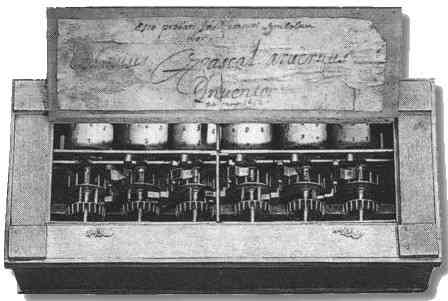
\includegraphics[width=0.4\textwidth]{./EtapaPrimeriza/imagenes/cp.jpg}
  \caption{Calculadora Pascalina (\href{https://www.tispain.com/2014/11/la-pascalina-la-primera-calculadora.html} {Primera Calculadora})}
  \label{cp}
\end{center}
\end{figure}

La máquina estaba compuesta de 8 ruedas dentadas conectadas entre sí con una numeración en ellas de 0 a 9 y una manivela que en función de de la forma de girarla indicaba la operación matemática que se quería realizar. Las 8 ruedas estaban distribuidas de la siguiente manera: dos de ellas se dedicaban a número decimales y las 6 restantes se utilizaban para números enteros. Esto significa que la calculadora te permitía hacer operaciones con número entre 0,01 y 999.999,99 lo que facilitaba un amplio rango de operaciones.\\

Lo curioso recae en el cómo se le ocurrió al joven Pascal inventar la calculadora. Era hijo de un funcionario recaudador de impuesto y en numerosas ocasiones ayudaba a su padre a redactar informes oficiales. Pascal pensó que si conseguía crear una calculadora ahorraría mucho tiempo y al mismo tiempo se aseguraba que los resultados eran correctos. Como resultado de ello apareció la primera calculadora mecánica de la historia dejando atrás instrumentos para contar como puede ser el ábaco.





\subsection{Isaac Asimov y las reglas de la robótica}

Isaac Asimov nacido en 1920 en la ciudad de Petrovichi, RSFS de Rusia. Con apenas tres años de edad su familia se trasladó a los EE.UU. y fue allí donde desarrolló su vida familiar, académica y laboral. A modo de curiosidad, señalar que debido a su precocidad intelectual sus padres decidieron falsificar su fecha de nacimiento para ingresar antes en un colegio neoyorquino. Una vez en la universidad se licenció e Químicas, Ciencias y Artes, Bioquímica y se doctoró en Filosofía. A lo largo de su vida tuvo dos esposas pero en ningún caso descendencia. Finalmente en 1992 fallece en Nueva York a causa del sida que había contraído en una transfusión sanguínea.\\

Durante su vida, Asimov destacó como escritor de ciencia-ficción y de divulgación científica. Fue en su libro \textit{"Yo robot"} donde este aventuró la relación que tendríamos los humanos con los robots, pero claro dichos robots no garantizaban la seguridad y prevención total de los riesgos. Es por ello que Asimov estableció las tres siguientes reglas de la robótica:

\begin{enumerate}
\item Un robot no hará daño a un ser humano o, por inacción, permitirá que un ser humano sufra daño.
\item Un robot debe cumplir las órdenes dadas por los seres humanos, a excepción de aquellas que entrasen en conflicto con la primera ley
\item Un robot debe proteger su propia existencia en la medida en que esta protección no entre en conflicto con la primera o con la segunda ley
\end{enumerate}

Señalar que Isaac Asimov era un adelantado a su tiempo y es que apostaba por la divulgación científica a través de la red. Es por ello que en 1988 aventuró la existencia de una plataforma como Wikipedia 13 años antes de que esta existiera. Además afirmaba la existencia en el futuro de plataformas como Skype, FaceTime o el desarrollo de coches autónomos, inventos que hoy en día son una realidad.



\subsection{Tortugas autónomas de Walter}

William Grey Walter nació en Kansas (EE.UU.) en 1910 y se trata de uno de los pioneros en el campo de la robótica, cibernética e inteligencia artificial. Sus estudios en neurología le llevaron a la investigación y desarrollo de inventos que eran capaces de medir ondas cerebrales y analizar el comportamiento del cerebro de una persona. Más concretamente, con la idea de que la conexión de neuronas o células cerebrales se podían ejecutar comportamientos complejos. Esto dio lugar a la construcción en 1948 y 1949 de las \textit{tortugas} Elmer y Elsie, respectivamente.\\

El nombre de tortugas se debe al caparazón de plástico que protegía al robot además de su lentitud en los movimientos. Solo estaban programadas para hacer dos misiones; esquivar obstáculos aunque no de una forma muy inteligente y volver a recargar su batería cuando esta estuviera cerca de agotarse. Las tortugas estaban formado por tres ruedas, una batería y una célula fotoeléctrica móvil que actuaba sobre el motor para decidir la dirección de los movimientos como lo hacen los actuales sensores.

\begin{figure}[H]
\begin{center}
  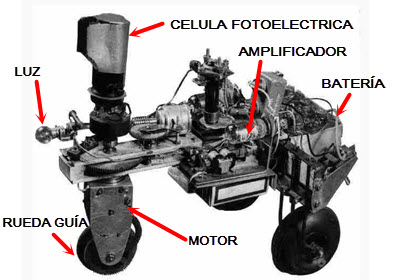
\includegraphics[width=0.5\textwidth]{./EtapaPrimeriza/imagenes/t1.jpg}
  \caption{Estructura de las Tortuga autónomas (\href{https://vonneumannmachine.files.wordpress.com/2011/05/elsie.jpg} {Von Neumann})}
  \label{t1}
\end{center}
\end{figure}


Walter fue el precursor de los robot aspiradores están tan de moda en nuestros días y que nos facilitan notablemente las tareas del hogar.


\subsection{El brazo robótico teleoperado de Goertz}


El primer brazo mecánico teleoperado se desarrollo por Raymond Goertz en 1949 y fue llamado \textit{M1}. El objetivo de su desarrollo era proteger del riesgo a los trabajadores mientras se permite la manipulación precisa de materiales o elementos radiactivos. Este es considerado el pionero en aplicar la técnica maestro-esclavo en sistemas de teleoperación. Más concretamente, en la máquina se consideran dos dispositivos diferenciados un brazo \textit{maestro} y otro brazo \textit{esclavo}. El brazo \textit{esclavo} se ubica dentro de un recipiente aislado en su totalidad y el brazo \textit{maestro} se sitúa en una sala de control y es el encargado de ejecutar ordenes que posteriormente el \textit{esclavo} reproducirá sobre el material radioactivo con notable precisión.

En 1951, Goertz diseñó una mejora en este brazo mediante la incorporación de una serie de poleas y cables de acero entre el brazo \textit{maestro} y el brazo \textit{esclavo} que proporcionaba mayor precisión en sus movimientos.\\

Durante el desarrollo de dicho brazo robótico, Goertz estableció uno principios que debía cumplir un brazo de este tipo y que aún se siguen aplicando a los robots quirúrgicos que se utilizan hoy en día. Los principios son los siguientes:

\begin{enumerate}
\item El movimiento del brazo \textit{esclavo} debe tener seis grados de libertad; tres de traslación, tres de rotación y uno de agarre.

\item El movimiento del brazo \textit{esclavo} debe estar acoplado al brazo \textit{maestro}.

\item Dicho acoplamiento debe ser bilateral, es decir, las fuerzas sobre el brazo \textit{esclavo} deben reflejarse en el brazo \textit{maestro} y los desplazamientos de producidos por el brazo \textit{maestro} deben producir el mismo desplazamiento sobre el brazo \textit{esclavo}.

\end{enumerate}


Seguidamente se muestra una imagen donde se puede observar el brazo robótico de Goertz descrito anteriormente.



\begin{figure}[H]
\begin{center}
  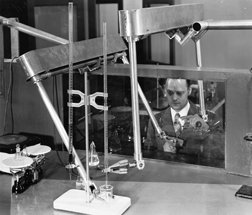
\includegraphics[width=0.5\textwidth]{./EtapaPrimeriza/imagenes/brazo.jpg}
  \caption{Brazo robótico de Goertz (\href{https://en.wikipedia.org/wiki/Raymond\_Goertz\#/media/File:Apf1-06395t.jpg} {Wikipedia})}
  \label{brazo}
\end{center}
\end{figure}


\subsection{Autónoma Universal de George Devol}

\textbf{George Devol} es conocido como el creador del primer robot industrial además de cofundador de la primera empresa robótica de la historia llamada \textit{\textbf{Unimation}} junto al empresario  Joseph F. Engelberger.

Este tenía el objetivo de crear una máquina que fuese fácilmente manejable y que trabajara de forma automática. Fue en el año 1948 cuando Devol patentó el prototipo de lo que más tarde se convertiría el primer robot de uso industrial. Este robot era un brazo que tenía la función de mover artículos de gran tamaño y gran peso en el ámbito industrial. Además era capaz de mover piezas a altísimas temperaturas y de hasta 225 kilos de peso.\\

Señalar que Devol y  Engelberger formaban un tándem perfecto, uno aportaba sus cualidades creativa y el otro las suyas empresariales. Esto les permitió fundar lo que fue la primera empresa robótica de la historia además de conseguir un contrato con la empresa \textit{General Motors} para instalar el brazo robótico en su fábrica de Nueva Jersey. Poco después, en 1968, firmó un contrato similar con la empresa japonesa de \textit{Kawasaki}. Señalar que en esa época las dos potencias industriales mundiales eran Japón y Estados Unidos y que por el contrario en Europa este tema estaba más estancado.

Más tarde, en 1978, Devol consigue mejorar este brazo robótico haciéndolo programable y multiarticulado, lo que permitía colocar las piezas en cualquier posición que se quisiese siempre que estuviese a su alcance. Este fue llamado \textbf{\textit{PUMA}} (\textit{Programmable Universal Machine for Assembly}).

Señalar que George Devol murió en 2011 a los 99 años de edad y que no se le puede negar la gran aportación a la industria que ha realizado ya que puso la primera piedra de la industrias robotizadas de la actualidad.






\subsection{Sputnik}

El programa \textbf{Sputnik} se trataba de una serie de misiones espaciales ejecutadas por la antigua Unión Soviética a finales de los años 50 y principios de los 60 del siglo pasado. El objetivo de este programa era probar la viabilidad de los satélites artificiales alrededor de la órbita de nuestro planeta.
Como curiosidad, señalar que el origen de la palabra \textit{Sputnik} proviene del ruso y significa \textit{satélite} o \textit{compañero de viaje}.
Durante este programa se lanzaron al espacio hasta 10 satélites diferentes. Seguidamente se describirán cada uno de ellos y el impacto que esto tuvo.\\


\textbf{Sputnik 1} [\ref{s1}] fue el primer satélite artificial de la historia el cual fue lanzado el 4 de Octubre de 1957. La importancia de este satélite recae en que fue el primer intento sin fallo de poner a orbitar alrededor de nuestro planeta un satélite artificial. Fue lanzado con el lanzador R-7 y este se encargó de analizar señales de radio que utilizaba para conocer la cantidad de electrones en la ionosfera. Estuvo en actividad durante 92 días y en la actualidad se puede visitar en la oficina neoyorquina de las Naciones Unidad.\\ 

\begin{figure}[H]
\begin{center}
  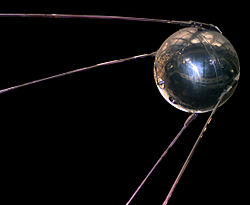
\includegraphics[width=0.5\textwidth]{./EtapaPrimeriza/imagenes/s1.jpg}
  \caption{Sputnik 1 (\href{https://es.wikipedia.org/wiki/Sputnik\_1\#/media/File:Sputnik\_asm.jpg} {Wikipedia})}
  \label{s1}
\end{center}
\end{figure}

Más tarde, se lanzó el \textbf{Sputnik 2} [\ref{s2}] el 3 de Noviembre de 1957. A diferencia del \textit{Sputnik 1}, este portaba un ser vivo en su interior. Aquí viajó la conocida \textit{Perra Laika}, y el objetivo de este lanzamiento era comprobar el efecto que causaba el medio espacial en un ser vivo. Regresó a La Tierra tras 162 días de actividad y en aquel momento de publicó que \textit{Laika} murió al regreso a nuestro planeta. Sin embargo, en 2002 fuentes rusas declararon que el animal había muerto al poco tiempo de ser lanzada a causa del estrés y el sobrecalentamiento del satélite.\\

\begin{figure}[H]
\begin{center}
  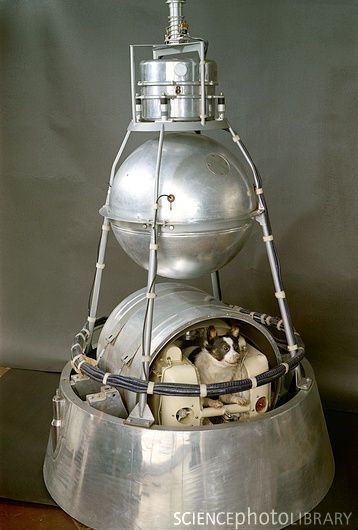
\includegraphics[width=0.3\textwidth]{./EtapaPrimeriza/imagenes/s2.jpg}
  \caption{Sputnik 2 con Laika en su interior (\href{http://www.alas-rojas.com/1-2.htm})}
  \label{s2}
\end{center}
\end{figure}

Fue el 3 de Febrero de 1958 cuando se intento lanzar el siguiente satélite, \textbf{Sputnik 3}. Esto quedó en un solo intento ya que fue fallido. Pero más tarde, se consiguió volver a lanzar esta vez ya correctamente. A pesar de que el sistema de grabación falló, transportó instrumentos para explorar la atmósfera superior y el espacio próximo.\\

\textbf{Sputnik 4} que fue lanzado el 15 de Mayo de 1960, fue el primer prototipo de nave espacial lanzada desde nuestro planeta y llevaba a bordo un maniquí de un hombre, un sistema de televisión y una cabina de soporte biológico. Pero un fallo en el sistema de guía la reubicó en una órbita más alta a la terrestre. Regresó el 5 de Septiembre de 1962, pero nada más tomar contacto con la atmósfera terrestre se desintegró. Algunas de sus piezas fueron encontradas al norte de los Estados Unidos, en Wisconsin.\\

Más tarde, el \textbf{Sputnik 5} se lanzó el 19 de agosto de 1960 y esta llevaba a bordo a los perros \textit{Belka} y \textit{Strelka} además de 40 ratones y numerosas plantas. La nave solamente permaneció en el espacio un día y todos los seres vivos regresaron con vida.\\

\textbf{Sputnik 6} fue enviado al espacio el 1 de Diciembre de 1960 con los perros \textit{Pchelka} y \textit{Mushka} junto a una serie de insectos, animales y plantas, y la cápsula no se consiguió recuperar. \\

Más tarde, el 4 de Febrero de 1961, \textbf{Sputnik 7} fue el primer intento de exploración de Venus. Sin embargo, el sistema de ignición tuvo un fallo y la sonda regresó a la órbita terrestre en lugar de tomar dirección a Venus.\\

Seguidamente, \textbf{Sputnik 8} se envió el 12 de Febrero de 1961 que transportaba la sonda Verena 1. Esta fue la primera nave espacial lanzada para sobrevolar el planeta Venus.\\

\textbf{Sputnik 9} fue una de las pruebas que tenían como finalidad iniciar los vuelos espaciales tripulados por humanos. Este completó un giro completo alrededor de nuestro planeta y volvió sin ningún problema lo que supuso un gran éxito.\\

Finalmente el \textbf{Sputnik 10}, al igual que el \textbf{Sputnik 9}, se trataba de una serie de pruebas con naves espaciales diseñadas para tripulación humana. Este portaba un perro, un astronauta ficticio y un sistema de televisión. Al igual que el anterior, se recuperó con éxito.

\begin{figure}[H]
\begin{center}
  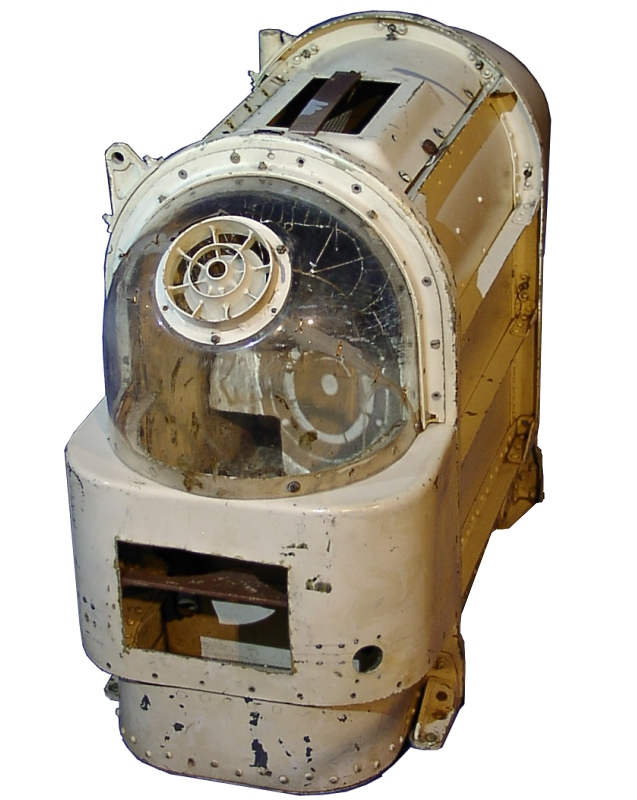
\includegraphics[width=0.3\textwidth]{./EtapaPrimeriza/imagenes/s10.jpg}
  \caption{Sputnik 10 (\href{https://es.wikipedia.org/wiki/Sputnik\_10\#/media/File:Russian\_space\_dog\_box.jpg} {Wikipedia})}
  \label{s2}
\end{center}
\end{figure}





\subsection{Robots Industriales de Generals Motors}


Por último, como fin a la etapa primeriza de la historia de la robótica vamos a hablar sobre \textbf{General Motors}, empresa norteamericana que destaca como fabricante mundial de vehículos. En 1957 se ofrece a esta empresa el conocido como Controlador Digital Modular, que está compuesto por máquinas de estado secuencial y que trabajan con procesadores centrales con desplazamiento de bits, que es el principio de lo que hoy conocemos como sistemas de control automático.\\

Pero sin duda el hito de \textit{General Motors} fue incorporar el primer robot industrial de la historia a sus instalaciones de Trenton, Nueva Jersey, en el año 1960. Este robot era un brazo robótico de 1800 kg de peso y que tenía la función de mover y colocar piezas metálicas de gran tamaño a grandes temperaturas. Señalar que este robot fue comprado a la empresa \textit{\textbf{Unimation}}, que como se ha comentado en apartados anteriores fue la primera empresa robótica de la historia fundada por  George Devol y el empresario  Joseph F. Engelberger.

Es en el 1978 cuando el robot \textit{PUMA}, desarrollado por la empresa de Devol y Engelberger, fue instalado en \textit{General Motors} para realizar tareas de montaje.




